%----------------------------------------------------------------------------------------
%	Metropolia Thesis LaTeX Template
%----------------------------------------------------------------------------------------
% License:
% This work is licensed under the Creative Commons Attribution 4.0 International License. To view a copy of this license, visit http://creativecommons.org/licenses/by/4.0/.
%
% Authors:
% Panu Leppäniemi, Patrik Luoto and Patrick Ausderau
%
% Credits:
% Panu Leppäniemi: abstract, def, cleaning,...
% Patrik Luoto: title page, abstract in Finnish, abbreviation, math,...
% Patrick Ausderau: initial version, style, table of content, bibliography, figure, appendix, table, source code listing...
%
% Please:
% If you find mistakes, improve this template and alike, please contribute by sharing your improvements and/or send us your feedback there: https://github.com/panunu/metropolia-thesis-latex
% And of course, if you improve it, add yourself as an author.
%
% Compiler:
% Use XeLaTeX as a compiler.

%----------------------------------------------------------------------------------------
%    ToDo
%----------------------------------------------------------------------------------------
% % % TÄRKEÄT
% % Translate "listing" in finnish (when inserting source code in the text)
% % Joku ifdef-tyyppinen vipu kieliversiolle (otsikot ja placeholdertekstit)
%    % Vaihtoehtona tietty erilliset filet suomelle ja enkulle, mutta
%    % tämä heikentää päivitettävyyttä (pitää aina muistaa korjata kahteen paikkaan).
%    % PA: I put CAPS comments where to switch depending on the language
% % Lisensointi (otsikkoon tekijä ja avoin lisenssi (esim. CC-BY, pohjan laatija
%   mainittava kommenttirivillä tjsp. [pohja ei ylitä teoskynnystä mutta kiva mainita].
%   PA: done
% % Projektin siirto Githubiin (siinä on issueträkkäys sun muut kivasti kunnossa) Vai?
%   %PA: done
% % Odotetaan 29.11.2013 asti äikänmaikkojen ja viestinnän mahdollisia kommentteja.
%   %done?
% %Reduce the vertical spacing for appendix in table of content
%   %done
%
% % % Vähemmän tärkeät
  % PNG:iden tilalle vektorigraffaa, jos vain löytyy kohtuuvaivalla

 
%----------------------------------------------------------------------------------------
%	THESIS
%----------------------------------------------------------------------------------------

\author{Uyiosa Imarhiagbe, Zoltán Gere, Albert Offei}
\title{Path follower(TM)}

\date{\today}
\def\metropoliadegree {Bachelor of Engineering}
\def\metropoliadegreeprogramme {Information Technology}
\def\metropoliaspecialisation {Smart Systems / Devices}
\def\metropoliainstructors {
Joseph Hotchkiss, Project Engineer\newline
Keijo Länsikunnas, Senior Lecturer}
\def\metropoliakeywords {Devices, Smart Systems, Embedded systems, Electronics}

%----------------------------------------------------------------------------------------
%	GLOBAL STYLES
%----------------------------------------------------------------------------------------

\documentclass[11pt,a4paper,oneside,article]{memoir}
%\usepackage[utf8]{inputenc}
%\usepackage[ansinew]{inputenc}
%\usepackage[T1]{fontenc}
%\usepackage[finnish]{babel} %IN ENGLISH, you can comment out or change this depending on your language
\usepackage[american]{babel} %IN ENGLISH, you can comment out or change this depending on your language
\usepackage{amsmath}
\usepackage{amsfonts}
\usepackage{amssymb}
\usepackage{fontspec}
\usepackage{tocloft}
%\usepackage{lipsum}
\usepackage{titlesec}
\usepackage[hyphens]{url}
\usepackage{mathtools}
\usepackage{wallpaper}
\usepackage{eso-pic}
\usepackage{datetime}
%\usepackage{lastpage} %other trick ;)
\usepackage{url}
\usepackage[amssymb]{SIunits}



\renewcommand{\dateseparator}{.}
%condition for adding or not space in TOC
\usepackage{etoolbox}
%for compact list
\usepackage{enumitem}
%for block comment
\usepackage{verbatim}
%for "easier" references
\usepackage{varioref}
%forcing single line spacing in bibliography
\DisemulatePackage{setspace}
\usepackage{setspace}
%including figure (image)
\usepackage{graphicx}
%change the numbering for figure
\usepackage{chngcntr}
%strike trough
\usepackage{ulem}
%euro symbol
\usepackage{eurosym}
%try to count
\usepackage{totcount}
%insert source code
\usepackage{listings}
\usepackage{caption}
\usepackage{color}
%force the width of a table instead of column
\usepackage{tabularx}

%NORMAL TEXT
%all text, title, etc. in the same font: Arial
%\setmainfont{Arial}
\setmainfont[
BoldFont=arialbd.ttf,
ItalicFont=ariali.ttf,
BoldItalicFont=arialbi.ttf
]{arial.ttf}
%line space
\linespread{1.5}
%\doublespacing
%margin
\usepackage[top=2.5cm, bottom=3cm, left=4cm, right=2cm, nofoot]{geometry}
\setlength{\parindent}{0pt} %first line of paragraph not indented
\setlength{\parskip}{16.5pt} %one empty line to separate paragraph
%list with small line space separation
\tightlists

%IMAGE - FIGURE
%the figures should be placed in the "illustration" folder
\graphicspath{{illustration/}}
%figure number without chapter (1.1, 1.2, 2.1) to (1, 2, 3)
\counterwithout{figure}{chapter}
%border around images
\setlength\fboxsep{0pt}
\setlength\fboxrule{0.5pt}
%caption font size
\captionnamefont{\small}
\captiontitlefont{\small}
%space after figure caption (and other float elements)
\setlength{\belowcaptionskip}{-7pt}

%TABLE
\counterwithout{table}{chapter}

%SOURCE CODE
%YOU NEED TO TRANSLATE THE CAPTION "Listing" in Finnish. 
%IN ENGLISH Nothing to do
\definecolor{darkgray}{rgb}{.4,.4,.4}
\definecolor{purple}{rgb}{0.65, 0.12, 0.82}
\lstset{
extendedchars=true,
captionpos=b,
caption=\footnotesize,
basicstyle=\singlespacing\ttfamily,%\small\fontfamily{"Courier"}\selectfont,
keywordstyle=\color{blue}\bfseries,
commentstyle=\color{purple}\itshape,
identifierstyle=\color{black},
stringstyle=\color{red},
showstringspaces=false,
showspaces=false,
numbers=left,
numberstyle=\footnotesize,
numbersep=9pt,
breaklines=true,
tabsize=2,
showtabs=false,
xleftmargin=1cm
}
%\counterwithout{lstlisting}{chapter}
%moved after begin document, otherwise does not compile

%TOC
%change toc title
%COMMENT OUT FOR ENGLISH
%\addto{\captionsfinnish}{\renewcommand*{\contentsname}{Sisällys}}
\renewcommand*{\contentsname}{Table of contents}
%remove dots
\renewcommand*{\cftdotsep}{\cftnodots}
%chapter title and page number not in bold
\renewcommand{\cftchapterfont}{}
\renewcommand{\cftchapterpagefont}{}
%sub section in toc
\setcounter{tocdepth}{2}
%subsection numbered
\setcounter{secnumdepth}{2}
\renewcommand{\tocheadstart}{\vspace*{-15pt}}
\renewcommand{\printtoctitle}[1]{\fontsize{13pt}{13pt}\bfseries #1}
\renewcommand{\aftertoctitle}{\vspace*{-22pt}\afterchaptertitle}
%spacing afer a chapter in toc
\preto\section{%
  \ifnum\value{section}=0\addtocontents{toc}{\vskip11pt}\fi
}
%spacing afer a section in toc
\renewcommand{\cftsectionaftersnumb}{\vspace*{-3pt}}
%spacing afer a subsection in toc
\renewcommand{\cftsubsectionaftersnumb}{\vspace*{-1pt}}
%appendix in toc with "Appendix " + num
\renewcommand*{\cftappendixname}{Appendix\space}

%TITLES
%chapter title
\titleformat{\chapter}
{\fontsize{13pt}{13pt}\bfseries\linespread{1}}
{\thechapter}{.5cm}{}
\titlespacing*{\chapter}{0pt}{.32cm}{9pt}
\titleformat{\section}
{\fontsize{12pt}{12pt}\linespread{1}}
{\thesection}{.5cm}{}
\titlespacing*{\section}{0pt}{14pt}{6pt}
\titleformat{\subsection}
{\fontsize{12pt}{12pt}\linespread{1}}
{\thesubsection}{.5cm}{}
\titlespacing*{\subsection}{0pt}{14pt}{6pt}


%QUOTE
\renewenvironment{quote}
  {\list{}{\rightmargin=0pt\leftmargin=1cm\topsep=-10pt}%
  \item\relax\fontsize{10pt}{10pt}\singlespacing}
  {\endlist}

%BIBLIOGRAPHY
%bibliography title to be "references"
%IN ENGLISH UN/COMMENT THIS 2 LINES
\renewcommand\bibname{References}
%\addto{\captionsfinnish}{\renewcommand*{\bibname}{References}}
%\addto{\captionsfinnish}{\renewcommand*{\bibname}{Lähteet}}
\makeatletter %reference list option change
\renewcommand\@biblabel[1]{#1\hspace{1cm}} %from [1] to 1 with 1cm gap
\makeatother %
\setlength{\bibitemsep}{11pt}

%count the appendices (since the chapter counter is reset after \appendix).
%! require to complie 2 times
\regtotcounter{chapter}

%TITLE PAGE
\newcommand\BackgroundPic{%
\put(0,0){%
\parbox[b][\paperheight]{\paperwidth}{%
\vfill
\centering
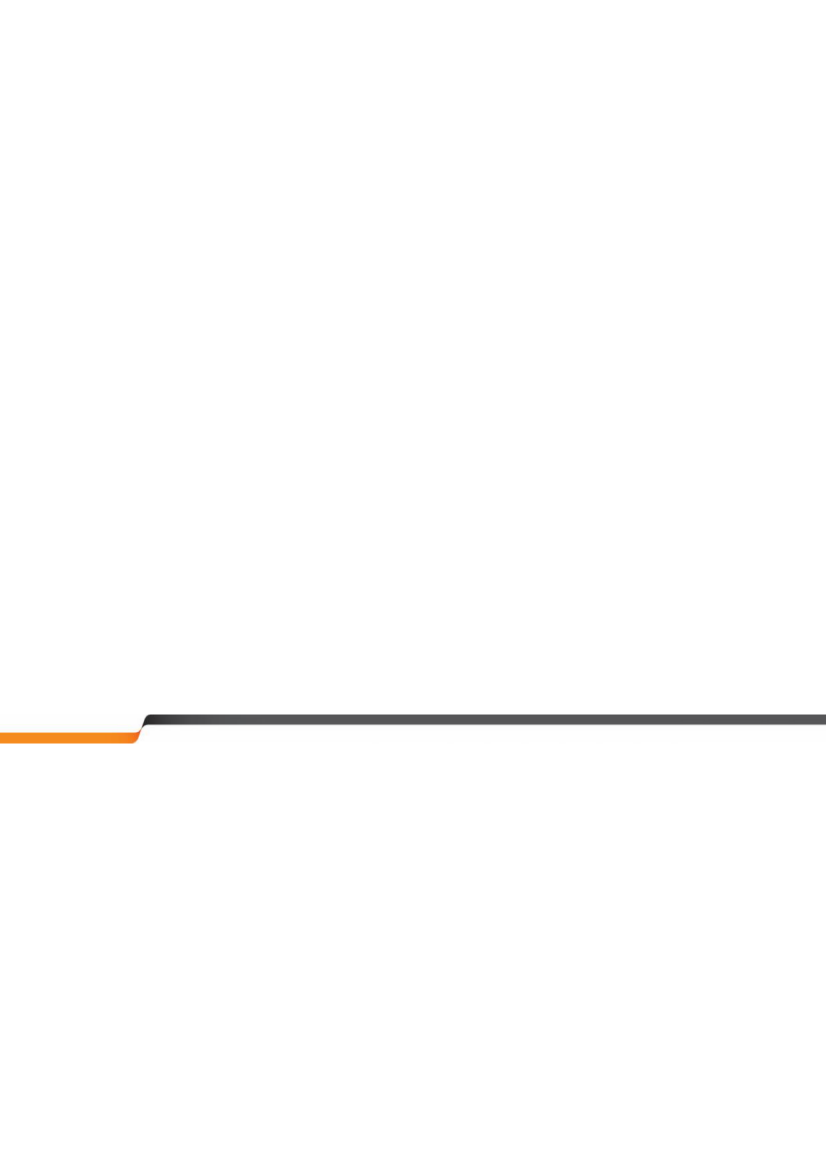
\includegraphics[width=\paperwidth,height=\paperheight,%
keepaspectratio]{viiva}%
\vfill
}}}


\makeatletter
\renewcommand{\maketitle}{
\thispagestyle{empty}
\ThisCenterWallPaper{1}{viiva}
%
\vspace*{9.5cm}
\tn{\LARGE \@author\\[0.75cm]\Huge \@title}\\[3.5cm]

\parbox{.7\linewidth}{\normalsize 
Helsinki Metropolia University of Applied Sciences\\[2pt]
\metropoliadegree \\[2pt]
\metropoliadegreeprogramme \\[2pt]
%Thesis\\[2pt]
\ddmmyyyydate\today}%to be checked date format? 

\ThisLRCornerWallPaper{1}{metropolia}
%
\clearpage
}
\makeatother

\makepagestyle{abstract}
\makeevenhead{abstract}{}{}{Abstract}
\makeoddhead{abstract}{}{}{Abstract}

%----------------------------------------------------------------------------------------
%	START OF THE CONTENT
%----------------------------------------------------------------------------------------
\begin{document}
\tracingall
\counterwithout{lstlisting}{chapter}

\newcommand\tn[1]{\textnormal{#1}}
\newcommand\reaction[1]{\begin{equation}\ce{#1}\end{equation}}

%page number always on the top right, clear the "chapter/section" head
\pagestyle{myheadings}
\markright{}
%clear chapter "title" foot page
\makeevenfoot{plain}{}{}{}
\makeoddfoot{plain}{}{}{}

%----------------------------------------------------------------------------------------
%	TITLE PAGE
%----------------------------------------------------------------------------------------

\maketitle
\newpage


%----------------------------------------------------------------------------------------
%	ABSTRACT
%----------------------------------------------------------------------------------------

\pagestyle{abstract}
\ThisLRCornerWallPaper{1}{footer}

\begin{tabular}{ | p{4,7cm} | p{10,3cm} |}
  \hline
  Author(s) \newline
  Title \newline\newline 
  Number of Pages \newline
  Date
  & 
  \makeatletter
  \@author \newline
  \@title \newline\newline
  \pageref{LastPage} pages + \total{chapter} appendices \newline %! if no appendices, risk to count total of chapter :D
  \@date
  \makeatother
  \\ \hline
  Degree & \metropoliadegree
  \\ \hline
  Degree Programme & \metropoliadegreeprogramme
  \\ \hline
  Specialisation option & \metropoliaspecialisation
  \\ \hline
  Instructor(s) & \metropoliainstructors
  \\ \hline
  \multicolumn{2}{|p{15cm}|}{
  	Project's aim is to develop an embedded software for Zumo robot control. This documentation covers the theoretical and practical principles required during development. Necessary mathematical, physical and electronic concepts also presented.
  } \\[14cm] \hline
  Keywords & \metropoliakeywords
  \\ \hline
\end{tabular}
\clearpage

%----------------------------------------------------------------------------------------
%	Acknowledgement ?
%----------------------------------------------------------------------------------------
%\chapter*{Acknowledgement}
%Thanks to my cats Sirnik and Masa for their continuous support.
%\clearpage

%----------------------------------------------------------------------------------------
%	TABLE OF CONTENTS
%----------------------------------------------------------------------------------------

\makeevenhead{plain}{}{}{}
\makeoddhead{plain}{}{}{}
\pagestyle{empty} %remove page number in toc (if longer than 2 pages)
\ThisLRCornerWallPaper{1}{footer}
\tableofcontents*
\pagestyle{empty} %remove page number in toc (if longer than 1 pages)
\ThisLRCornerWallPaper{1}{footer} %add footer image (if longer than 1 page)
\clearpage
\pagestyle{plain}

%list of figure, tables comes here...


%----------------------------------------------------------------------------------------
%    Lyhenteet / Abbreviation
%----------------------------------------------------------------------------------------

\pagestyle{empty}
\ThisLRCornerWallPaper{1}{footer}
\setlength{\parskip}{1cm}
\chapter*{Abbreviation}
\cftaddtitleline{toc}{chapter}{Abbreviation}{}
\begin{table}[h]
\setlength{\tabcolsep}{8pt}
\renewcommand{\arraystretch}{2}
\begin{tabular}{l p{12cm}}
AC	& Alternating current\\
AD	& Analog to digital (converter)\\
DA	& Digital to analog (converter)\\
DC	& Direct current\\
IR	& Infrared\\
NiMH	& Nickel-metal hydride\\
PID & Proportional, Integral, Derivate (control)\\
PWM & Pulse-width modulation\\

\end{tabular}
\end{table}

\newpage

%page number always on top right; also for chapter "title" page
\pagestyle{plain}
\makeevenhead{plain}{}{}{\thepage}
\makeoddhead{plain}{}{}{\thepage}

\setcounter{page}{1} %page 1 should be Introduction

%----------------------------------------------------------------------------------------
%	CONTENT
%----------------------------------------------------------------------------------------
\chapter{Introduction}
Project's aim is to develop embedded software which controls the Zumo robot behavior, manage its hardware resources and perform predefined tasks. Program change performed by reprogramming the firmware of the robot with a different program.

\chapter{Background}

First part of this chapter gives insight to theoretical electronic knowledge. The second part presents the electronic modules used in the robot and explains their components' operation.

\section{Pulse Width Modulation}
Pulse Width Modulation (PWM) is a modulation method used to encode information on a carrier signal. PWM is mainly used to empower electronic devices. As the modulated signal alternates between 0 and 1 the device gets an average power instead of continuous output. As a result the devices work in transition between OFF and ON states.\\
\begin{figure}[h]
	\centering
	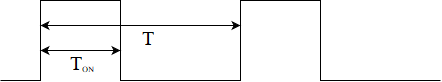
\includegraphics[width=12cm]{illustration/About_PWM}
	\caption[]{PWM cycle}
	\label{fig:aboutpwm}
\end{figure}
\\
Duty cycle means the length of ON state (T\textsubscript{on} in figure) during a full cycle (T in figure). The cycle length or frequency can move on wide spectrum from 1 Hz (1 cycle / second) to 10-100 kHz. (See appendix 1, Frequency)\\
In this project 1 cycle is exactly 2.56 ms long as 8 bit timer used. Therefore frequency is approximately 390 Hz. 0 value means no movement, brakes are on during the whole cycle.
\cite{wikipedia:PWM}


\section{PID controller}
Proportional-integral-derivative controller or PID controller is a control loop mechanism. The desired position called setpoint (SP). The measured position referred as process variable (PV). The difference of these values give the error value $ e(t) $. Based on this error value a new corrected position calculated. Calculation formula has 3 main parts each influencing differently the output.\\
\begin{figure}[h]
	\centering
	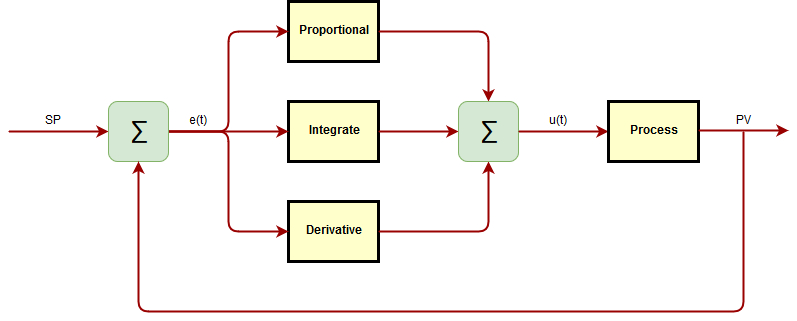
\includegraphics[width=12cm]{illustration/PID_controller}
	\caption[]{PID controller diagram}
	\label{fig:pidcontroller}
\end{figure}
\\
The proportional part is contributing linearly, greater current $ e(t) $ error value results in greater correction.
The integral part collects and integrates past error values. When this integrated error applied, it replaces the error deviation caused by proportional correction. As a result the quickly changing proportional correction replaced by a slowly changing integral correction and the function gets dampened.
The derivative part gives a future estimate based on the current changes in the function. It try to zero out the error change rate. Hence the derivative part cannot bring the error to zero.\\
\begin{align}
u(t) = K_{p}e(t) + K_{i} \int_{0}^{t} e(\tau)d\tau + K_{d} \dfrac{de(t)}{dt}
\end{align}
\\
This mathematical formula contains all three parts. If any part is not to be applied the respective coefficient values should be set to 0. Usually the integral, the derivative or both.
\cite{wikipedia:PID}
\cite{Lectures}

\section{Cypress CY8 modeling kit}
Cypress CY8CKIT is an Arm Cortex M3 based inexpensive prototyping kit. It includes a programmer and debugger modul, making development easier. It is programmed through USB connection. Output terminal is provided on UART port emulated over the USB connection. Software development and device firmware write performed with PSoC Creator IDE software provided by Cypress, the kits manufacturer.\cite{cy8ckit}

\section{Zumo robot}
The Pololu Zumo is a small size (less than 10cm) tracked base robot platform. The motors and controller are replaceable allowing customized builds. It includes a steel plate, mounted at the front to protect electronics and to provide capability to push objects. Power source is 4 pieces of AA battery.\cite{zumo}

\subsection{Power management}
The Zumo robot is powered by 4x 1,2V NiMH batteries. The micro controller runs with 5V and 0V. In order to protect the batteries form too low discharge the voltage is constantly measured. If the voltage drop low the user has to be noticed.\\
Because the micro controller operates with 5V, but the  well charged batteries can reach even 1.4V each (sum up in 5.6V) the actual voltage is scaled down to 2/3 (See appendix 1, Voltage division rule). This lowered voltage then directed to micro controllers AD converter unit.\cite{Lectures}

\subsection{Motor control}
Zumo's motors are 6V DC motors.
\begin{itemize}
	\item Idling: no acceleration and minimum force. Power input: 120mA at 6V.
	\item Stall: 1.6A / motor. Motor controller restricts current to 1.5A / motor.
	\item Speed: Run at 400 RPM. The installed gearbox's ratio is 75:1. The top speed is approximately 60 cm/s.
\end{itemize}
Motor controller unit connects batteries to both motors as instructed by control signals. Motor controller contains H-bridges (DRV 8835). DRV 8835 contains 2 bridges, thus capable to control 2 motors simultaneously.\\
\begin{figure}[h]
	\centering
	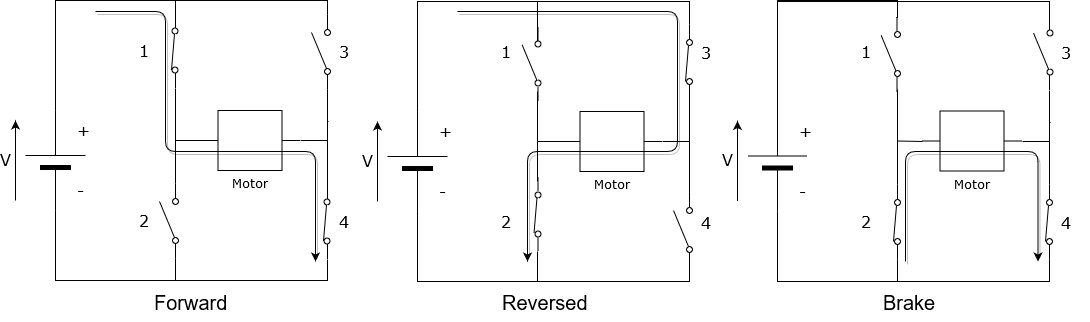
\includegraphics[width=15cm]{illustration/H-bridge}
	\caption{3 states of motor controller}
	\label{fig:h-bridge}
\end{figure}\\
Electronically there are 3 states the H-bridge can be.
\begin{itemize}
	\item Forward: direction set to 0, PWM set to 1
	\item Reverse: direction set to 1, PWM set to 1
	\item Brake: direction left as it was before braking, PWM set to 0
\end{itemize}
In brake mode the motor has changed to generator and shorted. In practice this means wheels locked. There is no mode when wheels can freely roll.
\cite{Lectures}

\subsection{Line detection sensors}
Zumo has 6 infrared light based sensor positioned at the front. Because IR light is out of visible spectrum, 2 red light led also placed on board. The IR led's light reflected from the surface under the robot back to the sensors. Amount of reflected light is measured using indirect AD conversion. Reflected light activates IR sensitive transistor which close circuit. The current flowing in the circuit is integrated in a capacitor until voltage reach defined level. Time to reach defined level is measured with a micro controller counter. If the surface is white, it has good reflection, so the big current charge the capacitor in short time.\\
The actual measurement happens in three steps.
\begin{itemize}
	\item Initial situation: Even when no measurement is happening some current might still flow eventually charging up the capacitor.
	\item Capacitor discharge: When the micro controller measurement pin gives 5V output, on both sides of the capacitor will be 5V. Consequently the capacitor discharge in 1\ldots2 \textmu s.
	\item Measurement: Micro controller measurement pin set to input and a timer is started. Capacitor starts to charge again as fast as the IR-sensitive transistor allows it. When capacitor charge reach about 2.5V, voltage at measurement point drops below 2.5V and the pin value turn to 0. Capacitor keeps charging up to 5V. Time to turn from 1 to 0 is measured.
\end{itemize}
Measurement procedure always takes 1 ms. Different sensors have different sensitivities. Environmental lighting also affects measurement as sun light contains plenty of infrared light.\cite{Lectures}

\chapter{Realization}

\section{The embedded software and mechanics}
Flow charts

\subsection{Voltage measurement}
Library for battery management is named \textless ADC\_Battery \textgreater . It is part of micro controller standard library and the source can be found in 'codegentemp' folder. Prior to use, it has to be initialized with ADC\_Battery\_Start() command.\\
Actual measuring is not instantaneous. The process is started with the  ADC\_Battery\_StartConvert() command.\\
Wait to finish measurement is achieved in one step:  ADC\_Battery\_IsEndConversion(ADC\_Battery\_WAIT\_FOR\_RESULT).
The actual value is queried with ADC\_Battery\_GetResult16() instruction. As the micro controller operates with 5V, measurement range is 0V - 5V. The AD converter is 12 bits unsigned therefore the return value is in 0 - 4095 interval. The formula of actual voltage:
\begin{align}
volts = \dfrac{AD code}{4095} * 5 * 1.5
\end{align}
. As mentioned in Chapter 2's Zumo robot section, battery voltage scaled down to 2/3. The trailing multiplication by 1.5 in the formula compensates this scale down.

\subsection{PID / Error calculation}

\subsection{Sharp turn calculation}
Lorem ipsum dolor sit amet, consectetur adipiscing elit. Aliquam aliquam aliquam purus, in ornare nulla imperdiet molestie. Nam tempus erat eu dui rhoncus et vestibulum mi elementum. Ut porttitor elit sit amet justo dignissim sit amet sagittis massa egestas. Mauris sed dolor eget dui fermentum sodales ut eu nibh. 

Quisque augue est, elementum ac porttitor non, porttitor ac orci. Donec hendrerit, ligula ac luctus egestas, sem dolor pretium nunc, sed vehicula magna diam a massa. Donec mattis, arcu et tempor mattis, risus tortor ultrices metus, nec sodales sem dolor eu elit. Nullam egestas enim at odio pellentesque bibendum. 

Donec et sapien ac leo condimentum vulputate id et tellus. Maecenas hendrerit malesuada interdum. Aenean dignissim sem faucibus elit congue faucibus id non risus. Morbi at dui non tortor pellentesque consequat non eget urna. Cras in sapien dui, a tincidunt velit.

\subsection{Motor speed programming}

\section{Timing}
Gantt charts

\begin{figure}[h]
	\centering
	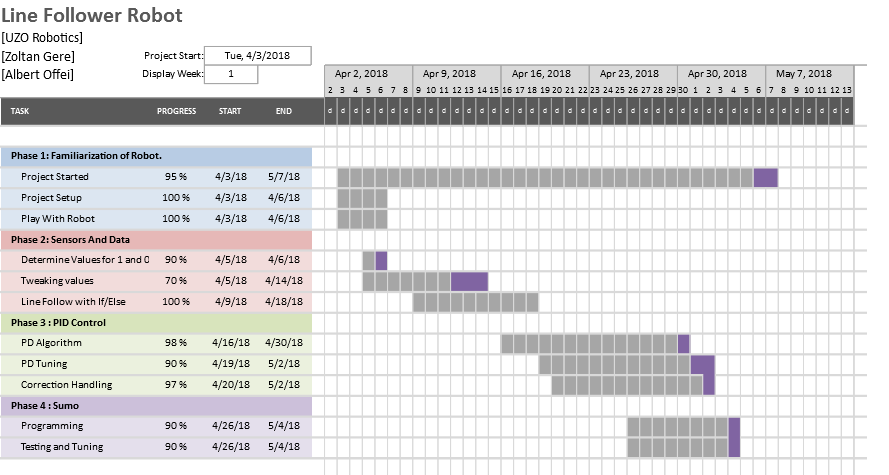
\includegraphics[width=15cm]{illustration/development_timeline}
	\caption{Development timeline}
	\label{fig:dev_timeline}
\end{figure}\\

Lorem ipsum dolor sit amet, consectetur adipiscing elit. Aliquam aliquam aliquam purus, in ornare nulla imperdiet molestie. Nam tempus erat eu dui rhoncus et vestibulum mi elementum. Ut porttitor elit sit amet justo dignissim sit amet sagittis massa egestas. Mauris sed dolor eget dui fermentum sodales ut eu nibh. 


\chapter{Conclusion}

What have been achieved, what can be improved.

\chapter{Latex formating helplet}
Lorem ipsum dolor sit amet, consectetur adipiscing elit. Aliquam aliquam aliquam purus, in ornare nulla imperdiet molestie. Nam tempus erat eu dui rhoncus et vestibulum mi elementum. Ut porttitor elit sit amet justo dignissim sit amet sagittis massa egestas. Mauris sed dolor eget dui fermentum sodales ut eu nibh. 

\section{Section}
Here is an example how to add biblio entry \cite{kopka:guide} using the \textquotedblleft cite\textquotedblright ~\cite[section 4.2]{tobias:book}. Note that a paragraph is added by forcing a new line.

And let also try the figure (see figure \vref{fig:latex-cover}) and internal reference (with label and ref or vref). The reference can be done to any label, for example why not to appendix \ref{appx:first} or to appendix \ref{appx:second}? To note, \LaTeX{} will place the figure to the best place (except with forcing). Let them float till the final of final edit\ldots ~then force them to not break a paragraph.%hugly hack... I'm sorry
\begin{figure}[h]
  \centering
  
\includegraphics[width=7.1cm]{LaTeX_cover}
  \caption{\LaTeX{} cover image (Copied from wikibooks.org (2012) \cite{wikibooks:latex}).}
  \label{fig:latex-cover}
\end{figure}

Let's also try a long quote:
From the Universal Declaration of Human Rights:
\begin{quote}
(1) Everyone has the right to education. Education shall be free, at least in the elementary and fundamental stages. Elementary education shall be compulsory. Technical and professional education shall be made generally available and higher education shall be equally accessible to all on the basis of merit.

(2) Education shall be directed to the full development of the human personality and to the strengthening of respect for human rights and fundamental freedoms. It shall promote understanding, tolerance and friendship among all nations, racial or religious groups, and shall further the activities of the United Nations for the maintenance of peace.

(3) Parents have a prior right to choose the kind of education that shall be given to their children. \cite[article 26]{un:udhr}
\end{quote}

\textit{Quisque augue} est, \textbf{elementum ac porttitor} non, porttitor ac orci. Donec hendrerit, ligula ac luctus egestas, sem dolor pretium nunc, sed vehicula magna diam a massa. Donec mattis, arcu et tempor mattis, risus tortor ultrices metus, nec sodales sem dolor eu elit.\vspace{-17pt} 
\begin{itemize}
\item \textbf{A small hack} with list
\item is to force the vertical space 
\item before and after the list
\end{itemize}
\vspace{-17pt} Nullam egestas enim at odio pellentesque bibendum. 

\subsection{Subsection}
Donec et sapien ac leo condimentum vulputate id et tellus. Maecenas hendrerit malesuada interdum. Aenean dignissim sem faucibus elit congue faucibus id non risus. Morbi at dui non tortor pellentesque consequat non eget urna. Cras in sapien dui, a tincidunt velit.

\subsection{Subsection with Math}
Donec et sapien ac leo condimentum vulputate id et tellus. Maecenas hendrerit malesuada interdum. Aenean dignissim sem faucibus elit congue faucibus id non risus. Morbi at dui non tortor pellentesque consequat non eget urna. Cras in sapien dui, a tincidunt velit.

Ionivahvuus lasketaan kaavalla.
\begin{align}
I&=\frac{1}{2}\cdot\sum z_i^2c_i \\
z_i&= \tn{ionin varausluku} \\
c_i&= \tn{ionin konsentraatio}
\end{align}
Aktiivisuuskerroin $\gamma_\pm$ lasketaan kaavalla.
\begin{align}
\log \gamma_\pm &= -\left|z_+\cdot z_-\right|A\cdot I^{\frac{1}{2}} \\
A &= \tn{0,509 (lämpötilassa 25\celsius}) \\
I &= \tn{ionivahvuus} \\
z &= \tn{ionien varaus}
\end{align}

\section{Section with Source Code}
Donec et sapien ac leo condimentum vulputate id et tellus. Maecenas hendrerit malesuada interdum. Aenean dignissim sem faucibus elit congue faucibus id non risus. Morbi at dui non tortor pellentesque consequat non eget urna. Cras in sapien dui, a tincidunt velit.

\vspace{-22pt}\begin{lstlisting}[language=PHP,caption={Descriptive Caption Text},label=testphp] 

<?php
$userName = $_POST["usern"];
//maybe not?
if ($userName){
	?>
	<h2>Hello <?php echo $userName; ?>!</h2>
	<p>your message got received.</p>
	<?php
}
?>
\end{lstlisting}\vspace{-22pt}


As see in listing \ref{testphp}: Donec et sapien ac leo condimentum vulputate id et tellus. Maecenas hendrerit malesuada interdum. Aenean dignissim sem faucibus elit congue faucibus id non risus. Morbi at dui non tortor pellentesque consequat non eget urna. Cras in sapien dui, a tincidunt velit.

\section{Section with Table}
Donec et sapien ac leo condimentum vulputate id et tellus. Maecenas hendrerit malesuada interdum. Aenean dignissim sem faucibus elit congue faucibus id non risus. Morbi at dui non tortor pellentesque consequat non eget urna. Cras in sapien dui, a tincidunt velit.

\begin{table}[h]
  \centering
  \caption{Some data}
  %IMPORTANT the caption must be before the tabular, so it will be on top of the table (there are other tricks to force it on top; but this one is straitforward).
  \begin{tabular}{| l | >{\centering\arraybackslash}p{.5\textwidth} |}
    \hline
    Test 1 & test 1234 test \\
    \hline
    Some more date comes here & with more values and if the text is very long it will disappear out of the box unless you force the column size :( \\
    \hline
  \end{tabular}
  \label{table:some_data}
\end{table}


As presented in table \ref{table:some_data}: Donec et sapien ac leo condimentum vulputate id et tellus. Maecenas hendrerit malesuada interdum. Aenean dignissim sem faucibus elit congue faucibus id non risus. Morbi at dui non tortor pellentesque consequat non eget urna. Cras in sapien dui, a tincidunt velit.

\begin{table}[h]
  \centering
  \caption{Another table with tabularx}
  \begin{tabularx}{.95\textwidth}{| l | >{\centering\arraybackslash} X |}
    \hline
    Test 1 & test 1234 test \\
    \hline
    Some more date comes here & with more values and if the text is very long it will disappear out of the box unless you force the table size :( \\
    \hline
  \end{tabularx}
  \label{table:some_data2}
\end{table}

As presented in table \ref{table:some_data2}: Donec et sapien ac leo condimentum vulputate id et tellus. Maecenas hendrerit malesuada interdum. Aenean dignissim sem faucibus elit congue faucibus id non risus. Morbi at dui non tortor pellentesque consequat non eget urna. Cras in sapien dui, a tincidunt velit.



%----------------------------------------------------------------------------------------
%   BIBLIOGRAPHY 
%----------------------------------------------------------------------------------------
\newpage
\bibliographystyle{vancouver}
%line space
%\singlespacing %removed otherwise the appendix are also single space
\begin{flushleft}
\begin{singlespacing}
\bibliography{biblio}
\end{singlespacing}
\end{flushleft}

%for conting the pages
\label{LastPage}~


%----------------------------------------------------------------------------------------
%   APPENDICES 
%----------------------------------------------------------------------------------------
%avoid that the last page of bib get appendix header
\clearpage
%start appendix
\appendix
%no page number for appendix in table of content
\addtocontents{toc}{\cftpagenumbersoff{chapter}}
%appendix sections and subsections not in table of content
\settocdepth{chapter}
%add "Appendices" in the table of content
\addappheadtotoc
%force smaller vertical spacing in table of content
%!!! There can be some fun depending if the appendices have (sub)sections or not :D
% You will have to play with these numbers and eventually copy the \pretocmd line on before some \chapter and force another number.
\addtocontents{toc}{\vspace{11pt}}
\pretocmd{\chapter}{\addtocontents{toc}{\protect\vspace{-24pt}}}{}{}

%have Appendix 1 (instead of Appendix A)
\renewcommand{\thechapter}{\arabic{chapter}} 

%each appendix restart page num to one
\setcounter{page}{1}
%special counter for appendix TODO: this is a ugly quick hack :( Should find a better way to count the page per appendix.
\newtotcounter{appx1}
%overwrite the header
\makeevenhead{plain}{}{}{Appendix \thechapter \\ \thepage (\stepcounter{appx1}\total{appx1})}
\makeoddhead{plain}{}{}{Appendix \thechapter \\ \thepage (\stepcounter{appx1}\total{appx1})}

\chapter{Physics}\label{appx:first}
\section{Frequency}
Frequency means for periodical functions (e.g. signals) the number of periods completed in 1 second. Unit of frequency is Hertz (Hz). For example 1 period in 1 second is 1 Hz. 10 period in 1 second is 10 Hz.

\section{Kinematics}

\section{Electricity}
\subsection{Voltage division rule}
Lorem ipsum dolor sit amet, consectetur adipiscing elit. Aliquam aliquam aliquam purus, in ornare nulla imperdiet molestie. Nam tempus erat eu dui rhoncus et vestibulum mi elementum. Ut porttitor elit sit amet justo dignissim sit amet sagittis massa egestas. Mauris sed dolor eget dui fermentum sodales ut eu nibh.

\section{Infrared light}
Infrared light (IR) is 700nm to 1mm section of light spectrum. The wavelength of IR is longer than that visible by human eye. This invisibility gives IR light wide range of purpose.

\clearpage % avoid that the last page of previous appendix get this header
\setcounter{page}{1} %restet to page 1 (you can't avoid this one (I think))
\newtotcounter{appx2} % to have the total for this appendix and not the previous one.
%overwrite the header
\makeevenhead{plain}{}{}{Appendix \thechapter \\ \thepage (\stepcounter{appx2}\total{appx2})}
\makeoddhead{plain}{}{}{Appendix \thechapter \\ \thepage (\stepcounter{appx2}\total{appx2})}

\chapter{Mathematics}\label{appx:second}

Note that every appendix will be a chapter.

Sorry for the ugly hack on how to count the total pages per appendix.

Of course with section and subsection.

\section{Appendix Section}

And you can cite \cite{tobias:book} stuff, it will go into the main bibliography.

Lorem ipsum dolor sit amet, consectetur adipiscing elit. Aliquam aliquam aliquam purus, in ornare nulla imperdiet molestie. Nam tempus erat eu dui rhoncus et vestibulum mi elementum. Ut porttitor elit sit amet justo dignissim sit amet sagittis massa egestas. Mauris sed dolor eget dui fermentum sodales ut eu nibh.

\subsection{With a Subsection}

Lorem ipsum dolor sit amet, consectetur adipiscing elit. Aliquam aliquam aliquam purus, in ornare nulla imperdiet molestie. Nam tempus erat eu dui rhoncus et vestibulum mi elementum. Ut porttitor elit sit amet justo dignissim sit amet sagittis massa egestas. Mauris sed dolor eget dui fermentum sodales ut eu nibh.

Quisque augue est, elementum ac porttitor non, porttitor ac orci. Donec hendrerit, ligula ac luctus egestas, sem dolor pretium nunc, sed vehicula magna diam a massa. Donec mattis, arcu et tempor mattis, risus tortor ultrices metus, nec sodales sem dolor eu elit. Nullam egestas enim at odio pellentesque bibendum. 

Donec et sapien ac leo condimentum vulputate id et tellus. Maecenas hendrerit malesuada interdum. Aenean dignissim sem faucibus elit congue faucibus id non risus. Morbi at dui non tortor pellentesque consequat non eget urna. Cras in sapien dui, a tincidunt velit.

\end{document}